%************************************************
\chapter{Introduction}
\label{chp:Introduction}
%************************************************

\section{Remote sensing in forestry }\label{sec:RemSensForest}

The development of remote sensing is strongly linked with the progress of flight -- across different realms from sky to space -- with a rather short scientific history.
Accordingly, the definition of the term \emph{remote sensing} itself has been evolving over the decades, and even today, scientists do not agree on one universal term. 
However, as a common basis in the scientific field, a general definition in the broad sense can be the following \parencite{Hildebrandt.1996, Franklin.2001}:

\begin{quote}
	Remote sensing \graffito{General definition \\ of remote sensing.} is the acquisition of information about objects or areas from a distance, 
	without making physical contact with them. 
	Further, the processing and analysis of the acquired data as well as the interpretation of the achieved results are essential parts of remote sensing.   
	The predominant aim in remote sensing applications is to achieve quantitative and qualitative information about the occurrence (pattern) of objects, 
	their current state as well as the changes over time. 
\end{quote}

\noindent When considering objects on the earth's surface, sensors for acquiring data are typically mounted on aircrafts or satellites. 
Generally, the sensors collect information by detecting electromagnetic radiation, which is emitted or reflected from the observed objects.
Two basic principles \graffito{Passive and \\ active remote \\ sensing systems.} of remote sensing data acquisition technologies can be distinguished:
(i) passive\index{passive remote sensing} remote sensing systems, which gather the natural energy that is emitted or reflected by the earth's surface, 
most commonly the reflected sunlight, and (ii) active\index{active remote sensing} remote sensing systems, 
which themselves emit electromagnetic radiation and measure the reflectance pattern returning from the earth's surface.

Examples for passive remote sensing systems include aerial photography or many earth observation satellite systems 
with multispectral sensors, \eg, Landsat or Sentinel 2. 
Radar and \ac{ALS} are examples of active remote sensing, with both technologies measuring the time delays between emission and return, 
allowing for the assessment of object location and other properties. 

From the advent of these new technologies, remote sensing allowed for the collection of data for vast and difficult-to-access areas. 
Thus, researchers and practitioners charged with mapping and analysis of natural environments like forests were early adopters to these data sets.
Today, \graffito{A large variety of remote sensing systems are used in forestry applications.} 
due to the fact of a widespread range of applications in forestry, including different scales in space (\ie, from needle to landscape to global) 
and time (\ie, from seconds to seasons to decades), a large variety of sensors are employed to best meet the research and practical necessities. 
The following list, which makes no claim to be complete, should facilitate the reader to get a brief overview
of important remote sensing systems and their primarily applications.  

\begin{description}
	\item [Earth observation satellite data:] Earth observation satellites\index{earth observation satellites} are purposely 
		designed to acquire data for characterizing environmental systems on a global scale.
		As the satellites continuously navigate around the globe, images covering vast areas can be recorded with high temporal repetition rates. 
		
		In environmental studies, data from earth observation satellites are typically utilized as information source to create maps of land cover and land use.
		Many of these satellite systems are designed for long-term global observations,
		 and the image series of these satellites recorded through time make them a primary data source when conducting time series analysis for assessing change pattern,
		 \eg, to quantify forest cover change etc. 
		Technically speaking, most of the applications dealing with satellite imagery can be assigned to the image classification domain. 

	\item [Aerial photographs:] Aerial photographs\index{aerial photograph} (airphotos) were pretty much the first largely available remotely sensed data source
		 and have been used manifold in forest research
		 and practice with different fields of applications (see section~\ref{sec:AerialPhotogrammetry}). For instance, these data found use in 
		 forest management planning or forest inventory in different regions.
		  
	\item[Airborne laser scanning:] Airborne laser scanning (\acs{ALS})\index{airborne laser scanning}\index{ALS|see {airborne laser scanning}}, 
		also referred to as airborne \ac{LiDAR}\index{LiDAR|see{airborne laser scanning}}, has been introduced to 
		forest research in the 1980s and 1990s \parencite{Nelson.2013},
		and is now widely acknowledged as the primary source to acquire information characterizing the three-dimensional
		forest vertical structure \parencite{Lim.2003, Maltamo.2014b}.
		\ac{ALS} can be used to measure the surface height of objects, \eg, trees, similarly to the photogrammetric measurements from stereo airphotos. 
		
		However, the laser pulses emitted from the measuring platform are able to penetrate through small gaps in the canopy, 
		and returns from leaves, branches, or stems
		additionally allow for the characterization of the vertical canopy structure. 
		Moreover, returns from the ground enable \ac{ALS} to even map the terrain underneath forest canopies with high accuracy. 
		This property, the availability to actually measure heights of objects within the canopy and of the ground -- which is invisible from optical 
		aerial or satellite images --
		made \ac{ALS} very attractive for forestry applications and stimulated enormous research efforts to fully explore the usability of these data. 

\end{description}



\section[Airphotos, ALS and aerial photogrammetry]{Aerial photography, 
	Airborne Laser Scanning and the renaissance of aerial photogrammetry}\label{sec:AerialPhotogrammetry}

\subsection{Acquisition principles for aerial photographs}

Typically, \graffito{Vertical airphotos \\ are perspective pictures of the underlying area \\
	with the camera pointing down vertically to the ground.} aerial photographs\index{airphoto|see{aerial photograph}}
are considered as perspective pictures of the underlying area taken with cameras mounted on aircrafts.
In most acquisition cases, vertical photographs are recorded, \ie, the camera is pointing vertically down towards the mapped area.
To cover larger areas of interest, aerial image acquisitions are planned and conducted in a block layout:
the aircraft is following a series of parallel flight lines, and photographs are taken such that they overlap to a specified amount in both directions 
along track (\emph{forward}) and across track (\emph{side}; see Figure~\ref{fig:vertAirPhoto}).

In this way, \graffito{Overlapping areas \\ of airphotos allow \\ for photogrammetric analysis.} 
each object within the study area is depicted from at minimum two different positions.
The overlapping parts of the images are referred to as the stereoscopic overlap areas, 
which can be analysed following the stereophotogrammetric measuring principle. This allows for 
the recovery of exact positions of surface points, \ie, estimating the three-dimensional coordinates of specific points or objects. 

\begin{figure}[!tb]
	\centering
	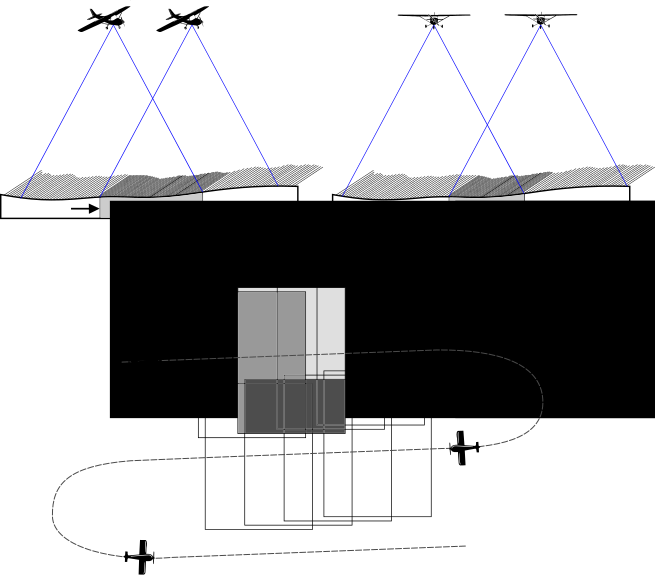
\includegraphics[width=0.8\textwidth]{Figures/vertAirPhoto/vertAirPhoto_v2} %scale for golden ratio 0.618
	\caption[Exemplary setting for aerial photograph acquisitions.]{Exemplary setting for aerial photograph acquisitions. 
		The typical overlaps of the images within flight lines (\emph{forward}\index{overlap!forward}) and across flight lines (\emph{side}\index{overlap!side})
		range between 60--80\,$\%$ and 20--40\,$\%$, 
		respectively (modified after \cite{vanLaar.2007} and \cite{AFL.2012}).}
	\label{fig:vertAirPhoto}
\end{figure}

\subsection{Early forestry related applications of aerial photography}

The use of aerial photography for mapping and monitoring forested landscapes can look back upon a long tradition \parencite{Hildebrandt.1996}.
Airphotos have been routinely interpreted for several decades by natural resource scientists and managers, 
most commonly to assist in the mapping of large areas and to inform forest inventory programs \parencite{Cohen.1996, vanLaar.2007, AFL.2012} . 

The very first documented trial for utilizing aerial photographs for practical forestry was undertaken as early as 1887, 
when photos taken from a balloon were used to sketch a map of forest stands close to Berlin in Germany \parencite{Hildebrandt.2010}. 
% Artikel im Berliner Tageblatt vom 10. September 1887. Überschrift „Die Verwendung der Ballonphotographie zu forstwirtschaftlichen Zwecken“
In subsequent years aerial photographs have been employed for forestry routine tasks throughout the world.
This development was especially promoted after the First World War when steerable aircrafts were available 
and aerial frame cameras\index{aerial frame camera} were invented.

Typical purposes of application \graffito{Airphotos have been used for mapping, \\ for support of forest inventory and management planning, 
	and for monitoring forest vitality.} 
include large scale mapping (\eg, 1:10\,000) and forest management planning for intensively managed forests 
(as common in many European jurisdictions) or in support of region-wide inventory programs with delineations 
of forest cover maps (like often necessary in North American regions). 
Further, the aerial imagery has been used for laying out and mapping forest road networks, 
and, especially with the advent of the colour-infrared\index{colour-infrared} film, for monitoring forest vitality and detecting areas damaged by,
\eg, storms or bark beetle infestations \parencite{Hildebrandt.1996}.

Whereas until today aerial photographs are used as one of the main sources of information for the aforementioned areas of application, 
the full potential of stereoscopic aerial photo-interpretation has not been unfold until the recent past. 
From the beginning of aerial photography, analogous taken pictures were the primary source of information
and a lot of manual processing was necessary prior to analysis. Stereo-interpretation was labour-intensive and required a high level of training.
Due to that, orthophotos were utilized for analysis in many applications instead of conducting expensive stereo photo-interpretation.
\textcite{Hildebrandt.1996} emphasized that even 100 years after the first application of airphotos in forestry, 
these data are seldom used for forest mensuration purposes or for forest site assessment. 

\subsection{Height assessment via stereophotogrammetry}\label{subsec:HeighAssessStereo}

The \graffito{Stereophotogrammetry allows for the measurement of 3d\index{3d|see{three-dimensional}} coordinates.} most valuable technological achievement of stereophotogrammetry\index{stereophotogrammetry} 
is the ability to actually measure the three-dimensional\index{three-dimensional} coordinates of objects, 
which can be identified in at least two overlapping images. 
Having this stereophotogrammetric measuring principle on hand, it seems logical, that tree height is the most important dendrometric attribute 
which can be assessed via stereo aerial photographs \parencite{Paine.2012}.

However, \graffito{For exact tree height measurements, tree top and base must be visible in the aerial photographs.} 
the exact measurement of tree heights is restricted to those trees, where both the tree top and base is visible in the photos. 
In dense forest stands, it actually is impossible to find ground points in the close vicinity to the trees of interest, 
in order to get the required elevation of the tree base.
This shortcoming when using aerial photogrammetry as sole remote sensing information source is one reason 
which impeded the broad use for tree height measurements -- and for assessing stand heights and related attributes of interest.   

Soon after the widespread integration of aerial photographs in forestry, 
researchers examined their usefulness for forest mensuration tasks,
in particular for determining growing stocks of forest stands.
Pioneer work was done by \textcite{Hugershoff.1933} and \textcite{Neumann.1933}.
They \graffito{Cross-sectional canopy profiles \\ can be used to approximate \\ growing stock.} introduced an approach 
based on continuous surface measurements and consecutive derivations of vertical canopy extents,
resulting in cross-sectional\index{cross-sectional} canopy profiles\index{canopy profile} of forest stands (Figure~\ref{fig:profile}). 
In their work, they could demonstrate that the cross-sectional areas of the canopy profiles were apparently related to the amount of 
timber volume at the site of the profile. \textcite{Spurr.1948} mentioned, that this method is especially useful when 
approaching uneven-aged stands, as variations in tree height and stand density are considered. 
By constructing multiple parallel cross-sectional profiles of the forest stand of interest, 
the \emph{growing space} describing the canopy volume could be constructed and used as proxy for growing stock.

\begin{figure}[bth]
	\centering
	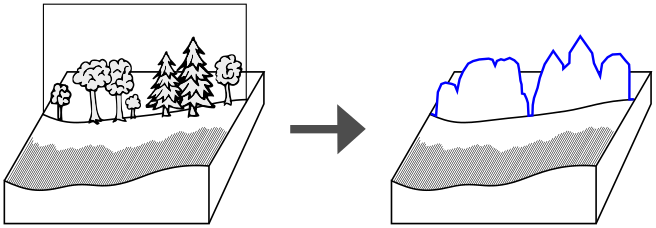
\includegraphics[width=0.80\textwidth]{Figures/Cross_Section/Cross-Section_A4_v2}
	\caption[Basic idea of the cross-sectional canopy profile derived from measurements of the three-dimensional
	forest canopy structure.]{Basic idea of the cross-sectional canopy profile derived from measurements of the three-dimensional forest canopy structure.  
		Detailed measurements of the outer canopy surface are achievable by both the \ac{DAP} and \ac{ALS} technology.
		However, photogrammetric measurements of the ground are restricted to gaps in the canopy. By contrast, active \ac{ALS}-measurements 
		allow for a detailed description of the terrain even for densely stocked forests. Thus, by combining 
		photogrammetric height measurements of the canopy surface and \ac{ALS} measurements of the ground, 
		detailed descriptions of actual forest heights become possible (modified after 
		\cite{Aldred.1985}, \cite{Nelson.1984} and \cite{Nilsson.1996}).}
	\label{fig:profile}
\end{figure}

However, due to the difficulty to determine these profiles with the analogue instruments available at that time, 
the method could not gain acceptance for widespread use. Meanwhile, researchers seized on that approach as the
development of better instruments facilitated the construction of canopy profiles based on stereo aerial photographs.
As an example, \textcite{Maclean.1984} measured cross-sectional canopy profile areas from stereoscopic aerial photographs with a stereoplotter,
and related these areas to timber volume data. They reported the relations to be highly significant, with regression $R^2$ values
ranging from 0.67 to 0.79. 

Nonetheless, \graffito{Drawbacks of photogrammetric tree height measurements impede extensive application.} 
two main aspects remained unsolved until the recent decades and hampered the further integration
of these approaches for assessing forest inventory attributes:

\begin{itemize}
	\item Conducting the methods described above with analogous instruments means a high effort in terms of manual
		work, when height measurements for the coverage of larger forest areas is desired.
	\item In dense forests, photogrammetric measurements of ground heights are restricted to irregularly distributed canopy openings.
		Interpolation of these sparse terrain height measurements results in inaccurate descriptions of the forest floor, especially for rough terrains.
		These errors in terrain height are propagated into tree- and stand-height measurements. 
\end{itemize}


\subsection{Airborne laser scanning in forestry}

As mentioned, the three-dimensional characterization of forest canopies by means of remote sensing tools 
has long been one of the top priority requests.
Over the course of the 1980s, \graffito{\ac{ALS} was introduced to forest research in the 1980s,
	focusing on assessing tree height and crown closure.} a new technology loomed on the horizon. 
\ac{ALS}\index{airborne laser scanning}  
was expected to provide detailed measurements of forest canopies, and in consequence, 
a lot of research concentrated on exploring the newly opened possibilities. 
Pioneer work was published, \eg, by \textcite{Nelson.1984, Aldred.1985}, who primarily focused on the assessment of tree heights and crown closure. 

\textcite{Maclean.1986} \graffito{Airborne \ac{LiDAR}-based cross-sectional profiles were regressed against timber volume.} 
picked up the ideas of \textcite{Hugershoff.1933},
and regressed timber volume against cross-sectional areas of canopy profiles of forests obtained by airborne profiling \ac{LiDAR} systems.
They elaborated on the mensurational significance of the variable \emph{cross-sectional profile area} as a remotely sensed wrapper variable
for total tree height, crown diameter and crown closure -- three sensitive indicators for timber volume. 
In their study, \textcite{Maclean.1986} demonstrated that the cross-sectional profile area is a very good indicator for 
the total amount of timber on a site.

\textcite{Nelson.1988b} tested a number of different laser metrics\index{metric} as predictor variables\index{predictor variable} 
to develop regression models\index{regression model} for timber volume and forest biomass.
The set of metrics comprised different measurements of forest height and canopy density. 
In their analysis, mean canopy height (calculated from the laser pulses and directly proportional to the canopy profile area)
proved to be best suited as independent laser variable for predicting timber volume and biomass, respectively.

As stated by \textcite{Baltsavias.1999c}, commercial \ac{ALS} systems became widely available during the 1990s.
These scanning systems were able to record area-covering measurements in contrast to the early profilers, 
and such provide much greater distributions of height samples.  
Research studies, in the beginnings conducted especially in the Scandinavian countries, 
examined the usability of the \ac{ALS} systems in forestry applications.

\textcite{Nilsson.1996} investigated how \ac{ALS} data acquisition parameters (laser beam footprint size and sampling density) affect 
stand height estimation.
He further explored the usability of these data for determining stand specific volumes in 
an even-aged stand dominated by Scots pine in Sweden. 
He found that the laser mean heights underestimated the ground measured mean tree heights, irrespective of beam divergence. 
In addition, he could demonstrate, for that study site, that there existed a linear relationship between 
stand volume and an \ac{ALS}-based metric including laser height and pulse density.

\textcite{Nsset.1997} used \ac{ALS} data to approximate the mean tree height of forest stands in Norway,
 dominated by either Norway spruce or Scots pine, and reported promising results.
 For the same stands, he assessed the accuracy of volume estimation
 by means of multiple regression\index{multiple regression} analysis, utilizing \ac{ALS} predictor variables describing 
 mean vegetation heights and canopy cover\index{canopy cover} densities \parencite{Naesset.1997}.
 He found that mean stand height and  mean height of the laser returns 
 (which might be regarded as per area unit of normalized canopy volume) were the most significant predictors for stand volume.
 The inclusion of the canopy cover metric, however, had a significant impact on the regression.
 
 Consecutive research was conducted, \eg, by \textcite{Magnussen.1998} or \textcite{Means.2000}, who reported on successful 
 \ac{ALS} applications in British Columbia and Oregon, respectively. The former study primarily focused on the
 exploration of a large set of possible predictor variables, which can be calculated from the airborne laser scanner measurements,
 for approximating forest stand heights. The latter demonstrated that \ac{ALS} data are capable to produce sound predictions
 for stand characteristics such as height, basal area and volume. Interestingly, 
 when using the \ac{LiDAR} metrics in stepwise regression analysis, height percentile metrics as well as canopy cover metrics 
 were selected for the final models of basal area and volume. \textcite{Means.2000} further proposed, that \ac{ALS} was now 
 a readily available source of information, which can be used to estimate stand characteristics over large areas -- 
 and after streamlining the process, maps displaying the spatial distribution of forest inventory attributes can be produced.
 
 Following \textcite{Means.2000}, \textcite{Nsset.2001} explored how accurately mean heights of the dominant trees and 
 numbers of stems can be predicted from \ac{ALS} metrics over young coniferous forest stands in Norway. 
In their regression analysis, they applied multiplicative models (in linear form with logarithmically transformed variables)
to develop the predictive models. The final models for dominant height and stem number achieved coefficients of determination ($R^2$) of 0.83 
and 0.42, respectively, with the finally selected predictors being the 90th height percentile plus the laser canopy density for the first and 
 canopy density solely for the second attribute. 
More important for practical use in forest management, \textcite{Nsset.2001} proposed a two-stage procedure for the prediction of 
mean dominant stand height. To do so, empirical relations between various \ac{ALS} metrics and tree heights measured in the field can be built
using small georeferenced sample plots. In the second stage, 
the forest area of interest gets divided into equal-sized cells with the single areas corresponding to the sample plots. 
The trained models can then be applied to provide estimates of tree heights for the respective cells,
and in consequence, for the stands throughout the forests. 
They evaluated their approach using 29 sample plots for training and 12 test stands, 
for which they report a mean height difference of 0.23\,m between
laser-derived and ground-truth stand heights. 

In his \citeyear{Nsset.2002} paper, \citeauthor{Nsset.2002} expanded the practical two-stage procedure for the prediction of six
forest inventory attributes: mean tree height, dominant height, mean diameter, stem number, basal area, and timber volume \parencite{Nsset.2002}.
He tested the procedure for young and mature forest stands following the same statistical methods as described in \textcite{Nsset.2001},
and concluded that the selected characteristics can be determined at the stand level with fairly high precision except for stem number.  
In subsequent years, this approach received much attention and was implemented to practical application
for large-scale forest inventory and management 
throughout different forest ecosystems \parencite{Nsset.2004b,Nsset.2004c,Hudak.2006,Li.2008,Hyyppa.2008,Woods.2011}.

The great relevance of \ac{ALS} in forestry applications, especially for the approximation of forest inventory attributes using the area-based approach
was confirmed by \textcite{White.2013}, who summarized the state-of-the-art approaches, methods, and data. In their best practices guide, 
they described the entire process for generating forest inventory attributes from \ac{ALS} data. 
Additionally, they discussed the use of different statistical methods for fulfilling the estimation tasks, 
including machine learning appraoches like \ac{RF}, which became popular recently. 
They further pointed to the fact, that there was currently increasing interest to the use of point clouds generated from high resolution 
digital aerial imagery, particularly for employing these data to generate estimates of forest characteristics in the same way as described above
for \ac{ALS} data.
 
\subsection{Digital images and processing capabilities}

During the last decade, aerial photography, and more specifically the photogrammetric evaluation capabilities of stereo airphotos,
experienced increased attention in forestry related remote sensing research activities \parencite{White.2013b,Holopainen.2015,White.2016}. 
This development has been instigated by a number of different factors \parencite{Leberl.2010,Haala.2012}:

\begin{itemize}
	\item ongoing improvements in camera technology, especially the introduction and further developments of digital aerial cameras;
	\item nation-wide availabilities of digitally recorded aerial imagery acquired within routine observation programs 
		run by the surveying authorities;
	\item inventions of advanced algorithms for image matching such as the pixelwise \ac{SGM} 
		and implementations to popular remote sensing software packages;
	\item rapid progress in hardware capacities enabling for the processing of large image blocks and the computed \ac{DAP} products.
	
\end{itemize}

\noindent The digital acquisition of airborne stereo photography achieved a breakthrough in administrative surveying in many jurisdiction, 
particularly in central and northern European countries.  Due to that, the availability of good quality photographs
with large degrees of overlap has been boosted in recent years.

Moreover, the development of new algorithms for image matching, which allow for the computation of dense photogrammetric height measurements
from stereo imagery, triggered increasing interest in digital airphotos as additional data source for retrieving 3d information.  
Thus, today \ac{DAP} is emerging as an alternate data source to \ac{ALS} for the three-dimensional characterization of forest structure.



\section{Prediction of forest inventory attributes}\label{sec:ABA}

As mentioned above, one major field of application for remote sensing in forestry is forest inventory.
Remote sensing data, particularly airphotos, have been commonly used to assist in inventory tasks, 
either as auxiliary data to facilitate inventory design or for other purposes. 

Nonetheless, with regard to both large-area inventories like \acp{NFI} or inventories purposely conducted for management issues
(\acsp{MFI}), the primarily used information is still gathered via ground based measurements at defined field sample plots.
Especially with regard to the intensively managed forest compartments as common in many European forest enterprises,
these inventories are the basis for both forest management planning and control. 

Most often, the ground plots are laid out systematically on a defined grid (\eg, 200\,m x 200\,m) throughout the forests, 
and cover specified areas (\eg, 500\,$m^2$), in order to achieve representative measurements \parencite[\eg,][]{Neufanger.2011}. 
Those field measurements allow for reliable assessments of the natural resources when considering the complete forest enterprises or 
specific strata. However, these inventories were not purposely designed to allow for statements at the level of the forest stand,
the primary unit of area for forest management. 

In contrast to the sample based measurements from terrestrial forest inventories, remote sensing provides data able to cover large areas.
By combining both data sources, the ground based measurements of the current forest state as response variable,
and the remotely sensed data providing explanatory information, in a statistical manner,
prediction models for forest inventory attributes by means of remote sensing can be trained and consequently applied to generate 
area-covering predictions \parencite{White.2013}. Next, these spatially explicit predictions can be used to assist in forest management, as they can provide information 
in a high spatial resolution.

One common method to accomplish the described necessity for approximating forest inventory attributes
and to consecutively predict their numerical values for wall-to-wall mapping is 
the \ac{ABA}\index{area-based approach}\index{ABA|see{area-based approach}}. 
This approach,
first proposed by \textcite{Naesset.2002b} for use with \ac{ALS} data in large-scale inventory, 
can be summarized in the processing steps as outlined in Figure~\ref{fig:ABA_method}.

\begin{figure}[bt]
	\centering
	\includegraphics[width=0.80\textwidth]{Figures/ABA_method/ABA_method_v3_crop}
	\caption[Schematic illustration of the area-based approach.]{Schematic illustration of the area-based approach for prediction 
		and wall-to-wall mapping of dendrometric forest inventory attributes.}
	\label{fig:ABA_method}
\end{figure}

  
 
In order to compute the statistical metrics summarizing the remotely sensed measurements of the forest canopy,
recorded measurements have to be translated into heights above ground before further use.
As mentioned above, one of the most beneficial aspects of \ac{ALS} is the possibility to simultaneously acquire height measurements 
from the vegetation and the underlying terrain. 
Thus, \ac{ALS} data can be directly converted to canopy heights above ground, and used in consecutive analysis.
By contrast, photogrammetrically computed heights only describe the outer surface heights -- this makes it necessary to employ 
ground heights from another source (\eg, \ac{ALS}), to arrive at the canopy heights above ground.

On a related note, when analysing and further processing these kind of 3d data, one has the option to either stick to the point data, 
or to translate the irregular measurements to rasterized surface models.
Following the first option, no loss in information has to be accepted, but specialized software is necessary for further processing.
On the other hand, following option two, which is compelling due to the ease in data storage and the availability of raster processing tools,
the operator has to select an appropriate spatial resolution for the computed rasters and has to keep in mind that by the rasterization, 
some detail information gets lost.

 





\section[DAP in forest inventory: current state]{Digital aerial photogrammetry in forest inventory applications: current state}\label{sec:DAP-current state}

As mentioned in the previous sections, different technical and methodological developments caused the returning interest
of forest scientists and practitioners to aerial photographs, in particular to \ac{DAP}. Therefore,
and due to the achievements made with \ac{ALS} data in the meanwhile, it is logical that this stimulated great interest in exploiting the 
digital imagery to generate \ac{ALS}-like characterizations of vegetation three-dimensional structure, especially as airphotos can be 
acquired at a fraction of the costs of \ac{LiDAR}.

The recent focus of work with \ac{DAP} data in forestry applications was particularly on its use in forest inventory.
This development is confirmed by the heavily increased number of published research dealing with these questions in recent years.
The following is an attempt to summarize the current developments and research results in this specific field,
as the aims and objectives of the work in hand are embedded in this general framework and 
especially focussed on the use of \ac{DAP} data for forest inventory tasks and to support forest management.
 
At the beginning of this decade, numerous studies focused on the comparison of \ac{DAP}-based height data 
and \ac{ALS} data for estimation forest inventory attributes following the \ac{ABA}. 
Initially, studies from Scandinavia were published \parencite{Bohlin.2012,Jarnstedt.2012,Nurminen.2013,Vastaranta.2013b},
investigating the predictive capabilities of \ac{DAP}-based height data for a set of attributes.
These studies were conducted for managed forests in flat terrain -- mostly even-aged stands with few species. 
 
 ERGEBNISSE DER STUDIEN ZUSAMMENFASSEN
 
 
Later on, research was also conducted for different and more complex forests, \eg, in central Europe \parencite{Straub.2013c} 
or the boreal of Ontario, Canada \parencite{Pitt.2014}. 
Under these more challenging conditions, the comparison of model performance for approximating forest inventory attributes
approved the results from the formerly conducted studies: the models using \ac{ALS}-based predictor variables
achieve somewhat higher accuracies than the models using \ac{DAP}-derived predictor variables.
  
 
 
\medskip
\emph{Zusammenfassung der bisherigen Studien zu ABA and DAP. \textbf{TABELLE}}
\medskip















% Research Aims and Objectives --> FERTIG!
\section{Research Aims and Objectives}\label{sec:Objectives}

The purpose of the presented work was to scrutinize digital aerial photographs, as regularly acquired by the Surveying Authorities nowadays, 
for use in forest inventory, forest planning, and forest management. 
During the course of the project, a range of applications was addressed and examined in different studies. 
The overarching aims of the presented studies were:

\begin{enumerate}
		\item Are \graffito{Overall aims of the studies.} digital aerial images acquired within the standardized
			administrative aerial surveys suitable to compute dense image-based point clouds
			or \acp{DSM} by means of image-matching techniques (\eg, \ac{SGM}), that characterize forest canopy surfaces with a sufficient level of detail?
		
		\item Can image-based outputs derived from digital airphotos, \ie, point clouds and raster-based surface models, 
			normalized to heights above ground using ALS-based \acp{DTM}, 
			be used to model key forest inventory attributes, \eg, mean or top height, basal area, and gross volume?
		
		\item Are repeated aerial image acquisitions and the derived image-based 
			\acp{CHM} capable to assess canopy height changes over time? 
\end{enumerate}

\noindent Against this background, more specific research objectives \graffito{Specific reseach objectives.} were formulated. 
We focused on these objectives in separate studies:


\subsection*{Stepper et al. \emph{Can. J. For. Res.} (2015)}

	\begin{itemize}
		\item application of \ac{SGM} to generate a very dense 2.5D point cloud that would provide a detailed characterization of the surface structure of the forest canopy;
		
		\item examination of several spectral features computed from the orthoimagery as additional explanatory variables
			for estimating gross volume $V$, in combination with height and structural variables derived from the image-based height data;
		
		\item comparative testing of \ac{RF} regression models vs. \ac{OLS} linear regression models to estimate $V$ at the plot level, as well as at the stand level;
		
		\item investigation of the effect of different sampling densities, \ie, systematically reduced numbers of terrestrial inventory plots,
			 on the accuracy and bias of the estimation of $V$.
	\end{itemize}

		
\subsection*{Straub \& Stepper \emph{Photogramm.\:Fernerkund.\: Geoinf.} (in press)}		
		
	\begin{itemize}
		\item adoption of the workflow as developed in \textcite{Stepper.2015b} for estimating a set of five forest inventory attributes -- stem density $N$, 
			basal area $G$, quadratic mean diameter $QMD$, volume $V$, and Lorey’s mean height $H_L$ -- using \ac{CHM}-based predictor variables and the \ac{RF} approach; 
		 
		\item evaluation of the impact of the prevailing forest type on the performance of models used to predict forest attributes.
			\Ie, study areas representing common broadleaf- and conifer-dominated forest environments in German	(beech- and
			spruce-dominated, respectively) were selected and predictive forest attribute models from both test sites were compared with respect to accuracy and bias.
	\end{itemize}


\subsection*{Stepper et al. \emph{Scand. J. For. Res.} (submitted)}		
 
 \begin{itemize}
 	\item investigation of predictive \ac{RF} models for the forest attributes $d_{100}$, $h_{100}$, and $V$. 
	 	Specifically, we study feature importance of predictor variables derived from \ac{SGM} point clouds and examine
	 	model performance by means of \ac{RMSE} and \ac{ME};   
 	
 	\item exploration of the spatial portability of forest attribute models to close-by forests, \ie, by means of large-area-covering aerial image data.
	 	The spatial transfer is validated at independent ground plots in neighbouring forest areas;	
 	
 	\item demonstrating the effect of training data coverage on model performance by systematically eliminating forest inventory plots for model training.
 \end{itemize}


\subsection*{White et al. \emph{Forests} (2015)}		

\begin{itemize}
	\item characterizing the differences between \ac{ALS}- and image-based point cloud metrics across a range of environmental conditions,
		defined by topographic slope and canopy cover;
	
	\item generation of area-based predictive models for Lorey's mean height $H_L$, basal area $G$, and gross volume $V$ from both sources
		of point cloud data and comparison of model outcomes in the context of the differences for the \ac{ALS}- and \ac{DAP}-derived metrics
		and in the context of different acquisition conditions for the imagery. 
\end{itemize}


\subsection*{Immitzer et al. \emph{Forest Ecol. Manag.} (2016)}

\begin{itemize}
	\item modelling gross volume $V$ using \ac{ACS} \ac{NFI} field data and \ac{WV2} stereo satellite imagery by implementing
		a multi-circle and multi-metrics approach for prediction at the pixel level;
	
	\item evaluating the explanatory power of spectral and height-related metrics computed from the multispectral WV-2 imagery and the image-based \ac{CHM};
	
	\item developing a wall-to-wall application method for the predictive models by using a moving-window approach.
\end{itemize}


\subsection*{Stepper et al. \emph{Forestry} (2015)}

\begin{itemize}
	\item application of \ac{SGM} to automatically compute image-based \acp{CHM} for two consecutive image data sets
		acquired as part of the regularly scheduled aerial image surveys in Bavaria;
	
	\item derivation and comparison of the \ac{PAI} of forest height computed from the two \acp{CHM} and
		two corresponding field inventory data sets at georeferenced ground plots;
	
	\item analysis of the \acp{PAI} in height for three height classes representing different successional stages -- \emph{youth}, \emph{full vigour} and \emph{old age}.
\end{itemize}









